% !TeX encoding = UTF-8
% !TeX program = pdflatex
% !BIB program = bibtex

%%% Um einen Artikel auf deutsch zu schreiben, genügt es die Klasse ohne
%%% Parameter zu laden.
\documentclass[english]{lni}
%%% To write an article in English, please use the option ``english'' in order
%%% to get the correct hyphenation patterns and terms.
%%% \documentclass[english]{class}
%%

\usepackage{booktabs}
\usepackage{pgfplots}

\pgfplotsset{width=12.5cm, height=4.4cm}

\begin{document}
%%% Mehrere Autoren werden durch \and voneinander getrennt.
%%% Die Fußnote enthält die Adresse sowie eine E-Mail-Adresse.
%%% Das optionale Argument (sofern angegeben) wird für die Kopfzeile verwendet.
\title[Which Rules Entail this Fact? - An Efficient Approach Using RDBMSs]{Which Rules Entail this Fact? \newline An Efficient Approach Using RDBMSs}
%%% \subtitle{From Facts to Rules using Relational Databases} % if needed
\author[Tim Gutberlet \and Janik Sauerbier]
{Tim Gutberlet\footnote{University of Mannheim, \email{tim.gutberlet@students.uni-mannheim.de}} \and
Janik Sauerbier\footnote{University of Mannheim, \email{janik.sauerbier@students.uni-mannheim.de}}}
\startpage{1} % Beginn der Seitenzählung für diesen Beitrag / Start page
\editor{B. K{"o}nig-Ries et al.} % Names of Editors
\booktitle{Datenbanksysteme f{"u}r Business, Technologie und Web (BTW 2023)} % Name of book title
\yearofpublication{2023}
%%%\lnidoi{18.18420/provided-by-editor-02} % if known
\maketitle

\begin{abstract}
Knowledge graphs (KGs) are used to store information about relationships between real-world entities in various fields. Learned rules over KGs describe patterns of KGs and allow for knowledge inference. In this paper, we focus on the problem of identifying all rules that entail a certain target fact given a KG and a set of previously learned rules. This can enable link prediction as well as help explain connections between rules and (potential) facts. Solving this problem time-efficiently for large rulesets and KGs is a challenge. To tackle this challenge, we propose an approach relying solely on RDBMSs including indexing, filtering and pre-computing methods. Our experiments demonstrate the efficiency of our approach and the effect of various optimizations on different datasets like YAGO3-10, WN18RR and FB15k-237 using rules learned by the bottom up rule learner AnyBURL. 
 
\end{abstract}
\begin{keywords}
Knowledge graphs \and Relational databases \and Link prediction \and Explainability.
\end{keywords}
%%% Beginn des Artikeltexts
\section{Introduction}
Many practically relevant large KGs are incomplete. Therefore, the prediction of missing or additional information, also known as link prediction, is highly relevant in contexts such as biomedicine \cite{OpenBioLink} or social networks \cite{SocialNetworks}. Rules describing patterns of KGs, which are learned by rule learning tools, can enable link prediction. The rule \((X, citizenOf, germany) \leftarrow (X, bornIn, mannheim)\) describes for example the implication that someone (\(X\)) born in Mannheim is a citizen of Germany. To determine the confidence of a potential new fact (link), one must know from which rules it can be derived. The confidence of a fact refers to the probability that a particular fact within the graph is correct. In our example: If we know that \(X\) was born in Mannheim it can help us determine the confidence of the fact that \(X\) is a citizen of Germany. Knowing the confidence is needed for rule-based link prediction models \cite{AnyBURL19}. Moreover, the confidence is used for building ensembles with link prediction embedding models \cite{RuleEmbeddingCombination1} and for improving link prediction embedding models \cite{RuleEmbeddingCombination2}. Therefore, it is important to identify all previously learned rules of a KG entailing certain target facts. Moreover, it is generally helpful to be able to explain the connections between rules and (potential) facts. To illustrate the performance of traditional RDBMSs in solving the problem in case of large rulesets and KGs, we create and analyze an efficient approach to this problem using PostgreSQL. As further discussed in the preliminaries, we are interested in the non-recursive application of rules and in finding all applicable rules for a given target fact. Therefore, our approach is limited to binary relations and conjunctive queries, in contrast to employing deductive databases. Our approach uses indexing, filtering and pre-computing methods tailored to the natural structure of a KG and its respective rules. We ran several experiments testing our approach on different KGs (YAGO3-10 \cite{YAGO3}, WN18RR \cite{WN18RR} and FB15k-237 \cite{FB15k-237}). Additionally, we show how different database setups impact the performance for different rule lengths. For the rule learning, we use AnyBURL, a fast bottom up rule learner for KGs \cite{AnyBURL19}.

\section{Preliminaries} 
A KG is a set of (subject, relation, object)-triples also called facts. There is a set of entities present as subjects and objects, as well as a set of relations in a KG. Here is an example KG with the entities \(peter\), \(anna\) and \(germany\) and the relations \(marriedTo\) and \(bornIn\).

\begin{equation*} \label{eq:knowledgegraph}
\textbf{KG} = \{(anna,marriedTo, peter), (peter,bornIn,germany)\}\end{equation*}

For our purposes, we are concerned about first-order logic Horn rules, which describe patterns of KGs. Here are two example rules. We capitalize the variables and lowercase the constants representing entities.

\begin{equation} \label{eq:rule_1}
(X, citizenOf, germany) \leftarrow (X, bornIn, mannheim) 
\end{equation} 
\begin{equation} \label{eq:rule_2}
(X, livesIn, germany) \leftarrow (X, marriedTo, A_1), (A_1, bornIn, germany)
\end{equation}

Each rule has a head (e.g., \((X, citizenOf, germany)\)) consisting of one atom and a body (e.g., \((X, 
bornIn, mannheim)\)) consisting of one or more atoms. A grounding of a rule assigns values to all variables of the rule, resulting in a ground rule. A true body grounding refers to a grounding of the body of a rule for which all (ground) atoms appear in the KG. The problem we are solving is identifying all rules that entail certain target facts based on the KG and a previously learned set of rules. This means we are interested in whether there exists a true body grounding and the head atom can be unified with the target fact. To illustrate the problem, think of the following target fact.

\begin{equation*} \label{eq:target_1}
\textbf{Target fact} = (anna, livesIn, germany)
\end{equation*}


Rule (\ref{eq:rule_1}) does not entail this fact because its head atom cannot be unified with the target fact.
The head of rule (\ref{eq:rule_2}) can be unified with the target fact by assigning \(X = anna\). Therefore, it would entail the target fact if \(\exists A_1 ((anna, marriedTo, A_1) \wedge (A_1, bornIn, germany))\). The KG contains the facts \((anna, marriedTo, peter)\) and \((peter, bornIn, germany)\). Together with the target fact, this results in a true body grounding for rule (\ref{eq:rule_2}) with \(X = anna\) and \(A_1 = peter\). Therefore, rule (\ref{eq:rule_2}) is part of the solution.

\section{Proposed Approach}

The given KG is stored in one table of the relational database (\textit{kg\_table} with columns \textit{sub} for subjects, \textit{rel} for relations and \textit{obj} for objects). The basic idea behind our approach is creating SQL queries which check whether a certain rule entails a certain target fact. Those individual queries are then combined using \textit{UNION ALL} operations over all rules, where the head can unify with the target fact. To improve this basic idea, we employ several optimizations listed below. Every rule has a specific rule ID which is returned if the rule entails the target fact. This would be the query for rule (\ref{eq:rule_2}) and the target fact given in the preliminaries:

\textit{\textbf{SELECT} rule\_id\_2 \textbf{FROM} kg\_table t0,  kg\_table t1 \textbf{WHERE} t0.sub = anna \textbf{AND} t0.rel = marriedTo \textbf{AND} t0.obj = t1.sub \textbf{AND} t1.rel = bornIn \textbf{AND} t1.obj = germany \textbf{LIMIT} 1;}

\subsection{Database Structure}
\label{database-structure}
Alternative to having one big table for all facts, our approach uses one table for each relation in the KG, with two columns for the subjects and the objects. 

To speed up the search and enable direct access to the table contents through B-trees, we employ unique clustered indexes. We duplicate the knowledge graph tables and use once (subject, object) as key and once (object, subject) as key for the indexes. Within the generated SQL statements, the tables with the order (subject, object) are used in case of a fixed subject. The tables with the order (object, subject) are used in the case of a fixed object or no fixed subject and object. This ensures that the indexes are used efficiently.

\subsection{Advanced Rule Pre-filtering} 
Firstly, we only consider rules that can unify with the target fact for the query. This can be done by naively testing each rule. However, it can also be done more efficiently. The easiest way is storing each rule under its head as key in a hash map. The head stays unchanged, but we use “\textit{X}” and “\textit{Y}” as variable descriptors. 

Let \textit{(s, r, o)} be a target triple with the entities \textit{s} and \textit{o} and the relation \textit{r}. Then we only use the rules stored under the keys \textit{(X, r, Y)}, \textit{(s, r, X)}, \textit{(X, r, o)} or \textit{(s, r, o)} for the query of the target triple. Additionally, when it is true that \(s=o\), we also use the key \textit{(X, r, X)}. Instead of looping through n rules naively in O(n), this allows for pre-filtering of the rules in O(1).

\subsection{Pre-computing of Expensive Rules}
\label{pre-computation}
As we will illustrate in our experiments (\ref{quintile-analysis}), certain rules result in way more cost in terms of execution time than others. To address that, we pre-compute a portion of those rules. To identify the most expensive rules, we gather an independent set of n target facts from the KG and run their queries with the \textit{EXPLAIN ANALYZE} command to get the execution time for the individual rule sub-queries. Afterward, we rank all rules which appear in the results by their average execution time multiplied with their number of appearances in the results. 

The top x\% of rules are then pre-computed, by calculating all potential assignments for variables in the rule head that form a grounding together with a set of facts from the KG. We then store these combinations in a table for the rule. If the subject or the object is a variable and the other one a constant, then the table only contains the column for the variable. For the implementation, we use indexed materialized views to \(SELECT\) from the KG with all the conditions we already know from the rule. Consequently, the \(CREATE\) statement for pre-computing rule (\ref{eq:rule_2}) and the query for the target fact from the preliminaries would be: 

\textit{\textbf{CREATE MATERIALIZED VIEW} view\_rule\_2 \textbf{SELECT} t0.sub \textbf{AS} sub \textbf{FROM} kg\_table t0,  kg\_table t1 \textbf{WHERE} t0.rel = marriedTo \textbf{AND} t0.obj = t1.sub \textbf{AND} t1.rel = bornIn \textbf{AND} t1.obj = germany};


\textit{\textbf{SELECT} rule\_id\_2 \textbf{FROM} view\_rule\_2  \textbf{WHERE} sub = anna \textbf{LIMIT} 1};

We exclude rules with one body atom, as pre-computing does not improve their performance. Beyond that, we limit the pre-computation to rules with two body atoms for illustration purposes, as rules with more body atoms incur a pre-computation time two orders of magnitude higher than rules with two body atoms.

\section{Experiments}
The goal of our experiments is to benchmark the performance of our approach on different datasets and rulesets, as well as to measure the effects of different optimizations. Furthermore, we analyze the execution time for individual rules. 

For the implementation of our approach, we used the open-source object-relational database system PostgreSQL. Additionally, we used Java with the PostgreSQL JDBC driver. The source code and datasets, we used for the experiments, can be found at https://github.com/timgutberlet/Which-Rules-Entail-This-Fact. We conducted all experiments on a Fujitsu Esprimo P957 (construction year 2017) with 32 GB RAM, 512 GB SSD, an Intel i7-7700 @ 3.6 GHz CPU and Ubuntu 22.04.1 LTS as an operating system. The rule learning with AnyBURL was mostly done with the standard configuration of AnyBURL-22 available at https://web.informatik.uni-mannheim.de/AnyBURL/. We only extended the limit of body atoms from one to three for acyclic rules to match the cyclic rules, as we do not intend to discriminate between them. This means the rulesets only include rules with up to three body atoms. The relations in the rule bodies are always extensional (defined by facts), never intensional (defined by other rules).

\subsection{Overall Performance}

\begin{table}[t]
\centering
\begin{tabular}{l|lll}
\toprule
 & AnyBURL - 10s & AnyBURL - 50s  & AnyBURL - 100s\\
\midrule
YAGO3-10 & 4.2 & 10.4 & 14.3\\
WN18RR & 34.8 & 65.0 & 77.3\\
FB15k-237 & 5.4 & 26.2 & 42.9\\
\bottomrule
\end{tabular}
\caption{Performance results (avg. execution time per target fact in ms)}
\label{tab:overall}
\end{table}

\begin{table}[t]
\centering
\begin{tabular}{l|lll|lll}
\toprule
 & \#entities & \#relations & \#facts of KG & 10s & 50s & 100s\\
\midrule
YAGO3-10 & 123,182 & 37 & 1,079,040 & 27k & 107k & 165k\\
WN18RR & 40,943 & 11 & 86,835 & 6k & 20k & 30k\\
FB15k-237 & 14,505 & 237 & 272,115 & 33k & 135k & 252k\\
\bottomrule
\end{tabular}
\caption{Dataset properties \& \#rules per ruleset learned by AnyBURL}
\label{tab:rules}
\end{table}

As illustrated in \Cref{tab:overall}, our approach works for different datasets and rulesets learned by AnyBURL. For every dataset, we learned rules for 10s, 50s, and 100s (\Cref{tab:rules}). We used the training sets as the KGs and the test sets as the target triples (3k-20k triples). The validation sets (3k-20k triples) were used as target triples to create the rule rankings to pre-compute the top 1\% most expensive rules with two body atoms.

\subsection{Ablation Study - Optimizations} 

\begin{table}[t]
\centering
\begin{tabular}{lll}
\toprule
Experiment & Avg. execution time (in ms) \\
\midrule
All optimizations enabled & 10.4\\
\midrule
Advanced rule pre-filtering disabled & 55.0\\
Tables for each relation disabled & 132.9\\
Indexing disabled & 1720.2\\
Pre-computing of expensive rules disabled & 14.1\\

\bottomrule
\end{tabular}
\caption{Ablation study of optimizations using YAGO3-10 \& 107k rules}
\label{tab:ablation}
\end{table}


For the ablation study in \Cref{tab:ablation}, we used YAGO3-10 as the benchmark dataset and the AnyBURL 50s ruleset (107k rules). We didn't analyze versions with multiple optimizations disabled due to very high execution times. The “tables for each relation” optimization described in \ref{database-structure} specifically reduces the execution time for long rules. We tested this, by measuring the average execution time of different rule lengths in the version where the “table for each relation” optimization is enabled versus the version where the “table for each relation” optimization is disabled. In both runs, the rule pre-computation was disabled. In this experiment, the execution time for rules with one body atom was reduced by 12\%, for two body atoms by 25\% and for three body atoms by 74\% when the “table for each relation” optimization is enabled. This might be caused by the increased use of the indexes during execution for longer rules.

\subsection{Rule Quantile Performance Analysis} 
\label{quintile-analysis}

\begin{figure}[t]
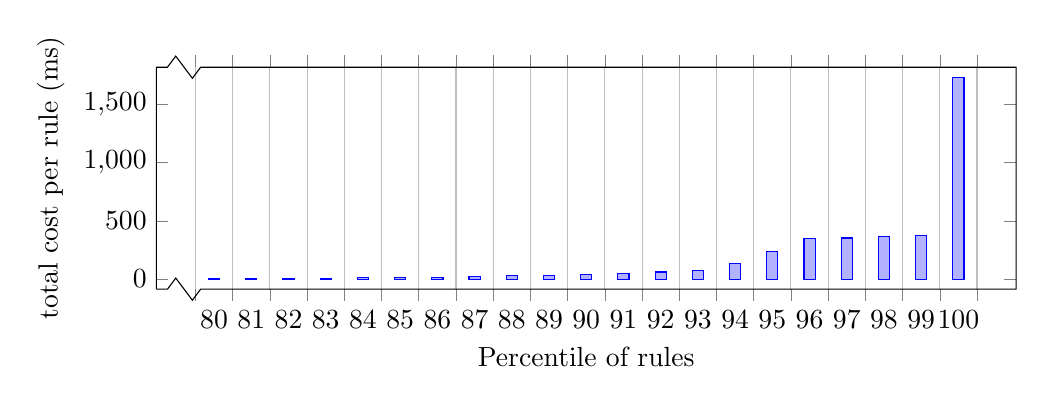
\begin{tikzpicture}
\begin{axis}[
	x tick label style={
		/pgf/number format/1000 sep=},
	ylabel=total cost per rule (ms),
        xlabel=Percentile of rules,
	enlargelimits=0.05,
	legend style={at={(0.5,-0.1)},
	anchor=north,legend columns=-1},
	ybar interval=0.3,
        axis x discontinuity=crunch
]

\addplot 
	coordinates {(80, 3.909)
            (81, 4.361) (82, 4.934)
            (83, 6.515) (84, 10.682)
            (85, 16.204) (86, 17.215)
            (87, 23.746) (88, 28.900)
            (89, 32.942) (90, 38.231)
            (91, 49.141) (92, 60.599)
            (93, 71.221) (94, 135.862)
            (95, 235.4) (96, 348.644)
            (97, 352.313) (98, 367.095)
            (99, 374.032) (100, 1731.569)
            (101, 0)};
\end{axis}
\end{tikzpicture}
\caption{Quantile performance analysis of rules using YAGO3-10 \& 107k rules}
\label{fig:quantile-analysis}
\end{figure}


The quantile analysis in \Cref{fig:quantile-analysis} is based on the total cost per rule after using the validation set as target triples, as described in \ref{pre-computation}. The total cost per rule is calculated by multiplying the number of appearances with the average execution time. Here, the number of appearances is a count for how often a rule appears as a result of the queries for all target triples. It indicates that only few rules incur a major share of the cost. The most expensive rules are predominantly rules with two variables in the rule head and two or three body atoms. Excluding those rules (978 rules) reduced the average execution time for YAGO3-10 \& the AnyBURL 50s ruleset (107k rules) to 0.14 ms per query using all optimizations. In the given example (YAGO3-10 \& 107k rules), we achieved an 98.8\% execution time reduction for the pre-computed rules. The pre-computation took 15 minutes. This reduced our average execution time from 14.1 ms to 10.4 ms, as illustrated in \Cref{tab:ablation}.


\section{Conclusions}

%
% the environments 'definition', 'lemma', 'proposition', 'corollary',
% 'remark', and 'example' are defined in the LLNCS documentclass as well.
%

We have designed an efficient approach for finding all rules that entail a certain target fact given a knowledge graph and a set of previously learned rules. Our experiments specifically demonstrate the effect of indexing, filtering and pre-computing methods. Potential next steps include a further analysis of our approach on various datasets, an empirical comparison of different database technologies (particularly triplestores and deductive DBMS), exploring the use of multithreading, investigating the use of multidimensional indexes and creating a dedicated solution only using the main memory.

\textbf{Acknowledgement.} This paper would not have been possible without the exceptional support of our supervisor, Prof. Dr. Rainer Gemulla.

%%% Angabe der .bib-Datei (ohne Endung) / State .bib file (for BibTeX usage)
\bibliography{references} %\printbibliography if you use biblatex/Biber
\end{document}
